\chapter{Design}
\label{sec:design}

% Ist das zentrale Kapitel der Arbeit. Hier werden das Ziel sowie die eigenen
% Ideen, Wertungen, Entwurfsentscheidungen vorgebracht. Es kann sich lohnen,
% verschiedene Möglichkeiten durchzuspielen und dann explizit zu begründen,
% warum man sich für eine bestimmte entschieden hat. Dieses Kapitel sollte -
% zumindest in Stichworten - schon bei den ersten Festlegungen eines Entwurfs
% skizziert werden. Es wird sich aber in einer normal verlaufenden Arbeit
% dauernd etwas daran ändern. Das Kapitel darf nicht zu detailliert werden,
% sonst langweilt sich der Leser. Es ist sehr wichtig, das richtige
% Abstraktionsniveau zu finden. Beim Verfassen sollte man auf die
% Wiederverwendbarkeit des Textes achten.

% Plant man eine Veröffentlichung aus der Arbeit zu machen, können von diesem
% Kapitel Teile genommen werden. Das Kapitel wird in der Regel wohl mindestens 8
% Seiten haben, mehr als 20 können ein Hinweis darauf sein, daß das
% Abstraktionsniveau verfehlt wurde.

\ldots design \ldots

\todo{write design}

In this chapter, I will explain the design of the TEE software and how a system
that utilized my TEE prototype looks. The design tries to mitigate the risk of
covered side channels by fully excluding them on an architectural base.\\

In the first section, I will describe the general system and usage of the TEE
prototype implementation. The second section of this chapter
(\ref{sec:30:system_description}) describes how different parts of the TEE system
are designed with section~\ref{sec:30:tee_kernel}  explaining the TEE kernel in
more detail. In section~\ref{sec:30:attack}, I review different attack vectors
and define attacks against which the TEE prototype has to defend itself.

\section{Environment}
\label{sec:30:environment}

I decided to implement the prototype for processors implementing the Intel Alder
Lake microarchitecture. In particular, I used the Intel Core i7 13700k processor
as a test vehicle. Because Intel and AMD use different address schemes for their
performance measurement extensions, the prototype will be bound to processors of
the chosen microarchitecture. These processors support the Intel Hyper-threading
feature that makes utilization of unused physical resources for a second logical
threat available. Because these sibling threats use the same physical resources,
they pose a security risk in the environment. For example,  sibling threats
compete for resources such as L1 Cache\todo{cite}, which could leak information
between threads\todo{cite} and denial of service through the competition.
Because of this, I decided to limit the environment and not use the
Hyperthreading feature.\\

Furthermore, the primary purpose of this work is to evaluate the feasibility of
a PMC-based monitoring approach. For simplicity, I will assume that I will be
able to install the TEE management software without being exposed to malicious
software. Features such as SecureBoot\todo{cite} support this assumption. The
prototype will, therefore, implement features to protect the running TEE.
Creating a trusted bootloader that is able to install the TEE in a trusted way
is left for future work.\\

For cryptographic key generation and as a hardware root of trust for
measurement, the prototype requires the presence of a TPM.


\section{System description}
\label{sec:30:system_description}

\begin{center}
    \begin{figure}
        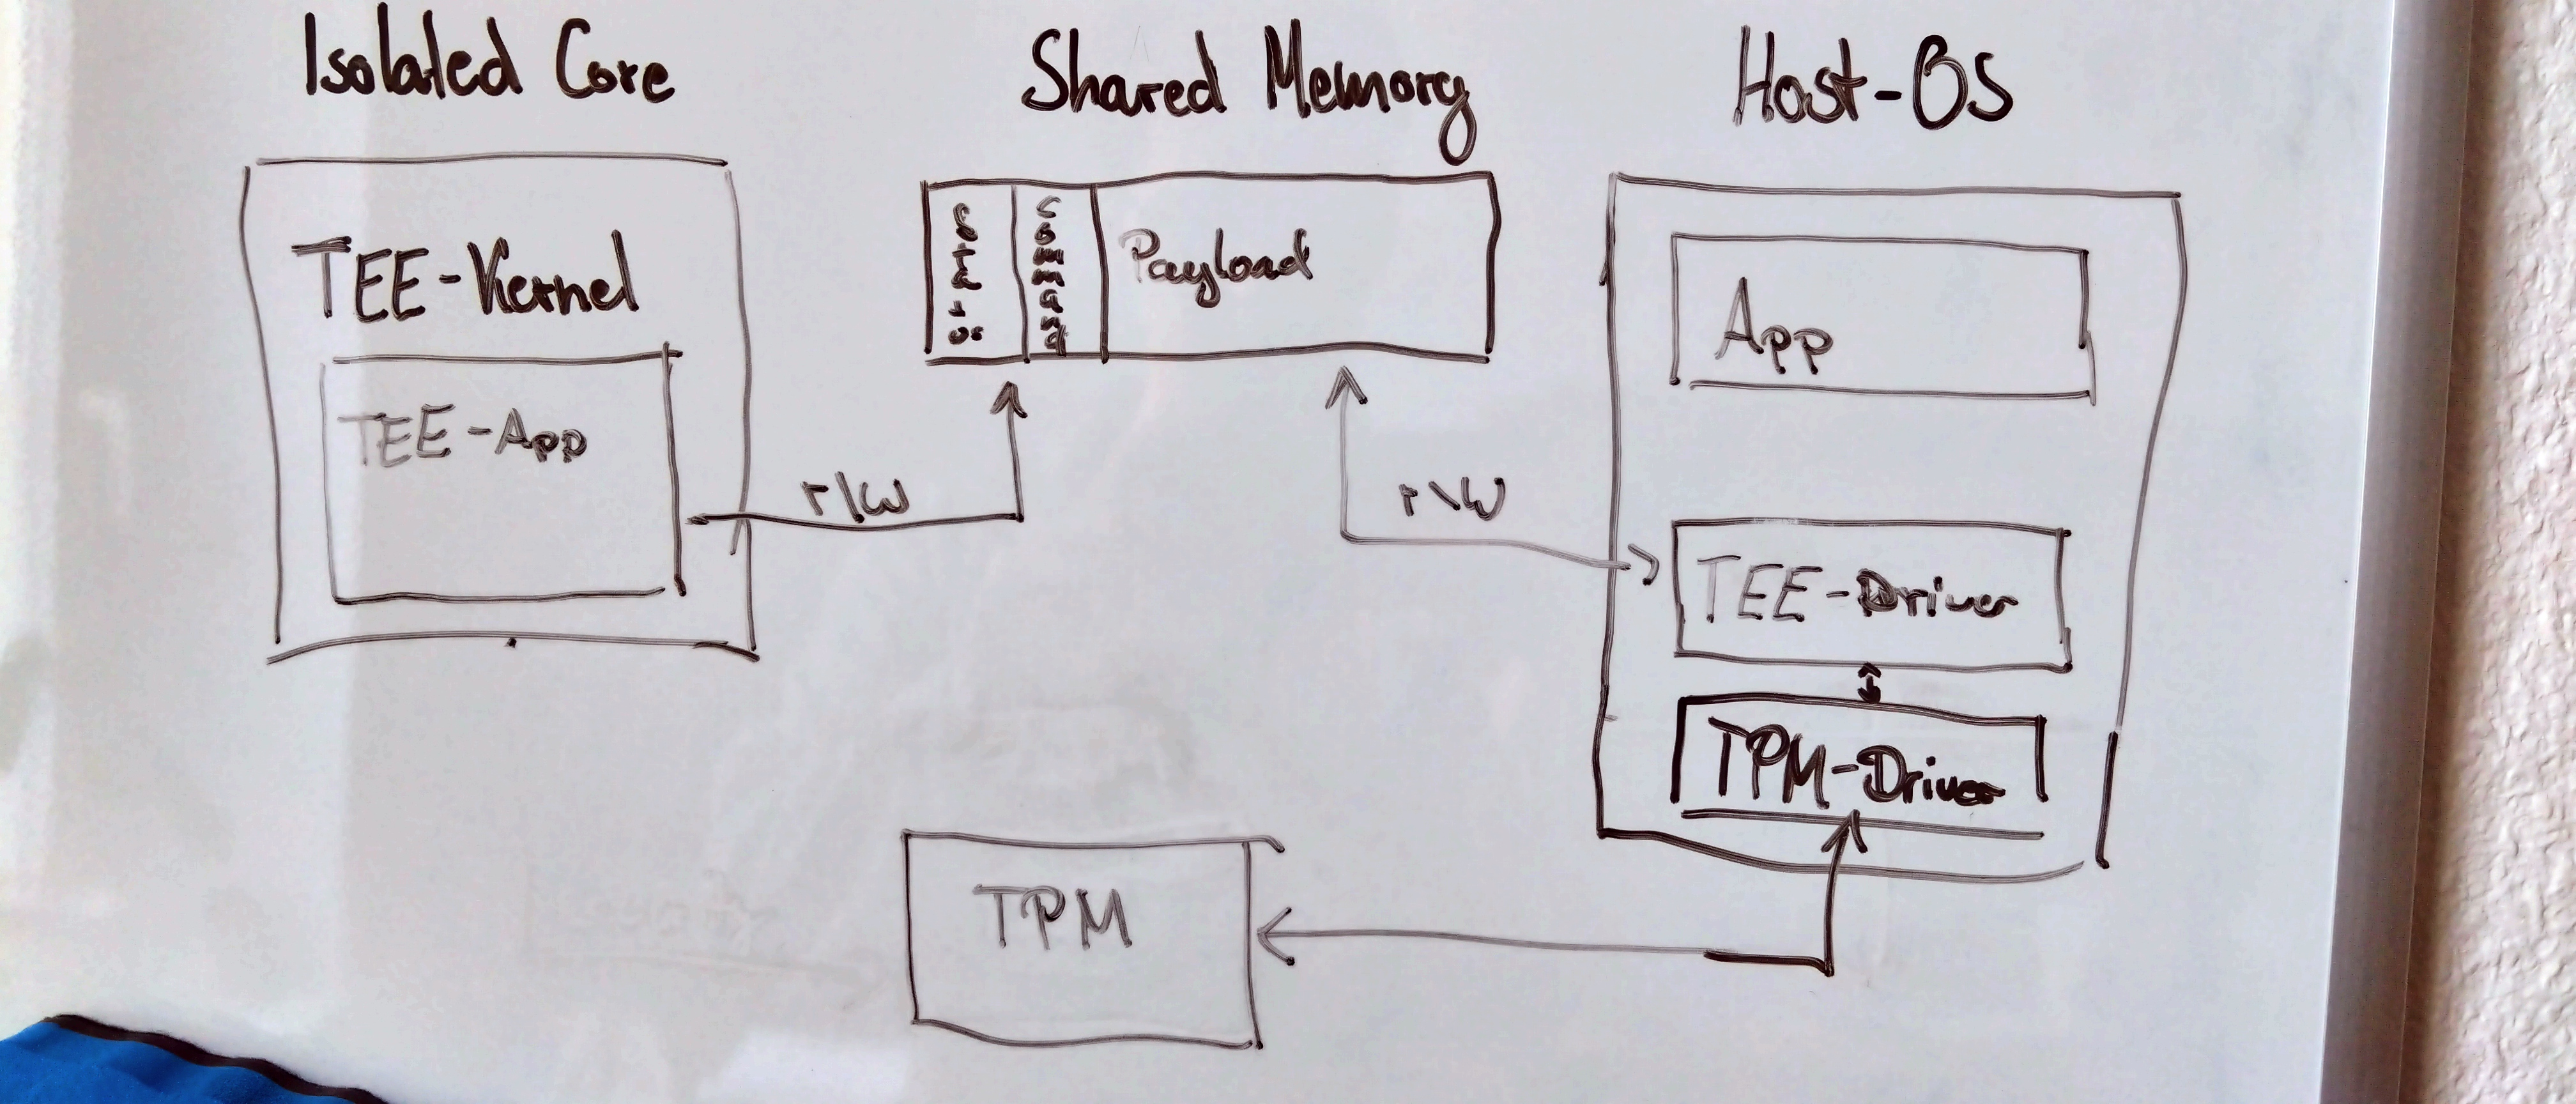
\includegraphics[width=.8\textwidth]{images/architecture.JPG}
        \caption{Components of the TEE system}
        \label{fig:30:tee_system_design}
    \end{figure}
\end{center}

A complete system that utilizes my TEE prototype is shown in
figure~\ref{fifig:30:tee_system_design}. The system consists of two privileged
software pieces: the TEE kernel and the host OS. Both run next to each other on
the same physical CPU package and cooperate to some extent with each other.\\

The host OS is a general-purpose operating system that runs user space
applications and offers services to those applications through an interface that
can communicate with the TEE kernel. Communication and management of a TEE and
its app Alication are implemented by the host OS through a driver. The host also
sets up the isolated core and shared memory communication path in the prototype.
\\

The TEE kernel, on the other hand, is responsible for setting up the environment
in which isolated trusted applications run. It manages the resources and brings
the CPU core into a state that can execute services. It additionally sets up a
communication path through shared memory. This shared memory must be known by
both the host OS and the TEE kernel.\\

Once booted with Secure boot, the TEE kernel can take ownership of the TPM and
use it as a hardware root of trust. With an x.509 certificate chain, the TEE can
create reports about its state. For this, the TEE kernel asks the TPM to create
a certificate and bind it to the TEE's signing key. Outstanders can then check
the validity of the certificate by verifying the key chain of the x.509 PKI.


\section{TEE kernel}
\label{sec:30:tee_kernel}

The TEE kernel must manage all resources available to the  TEE and Implements
mechanisms to enforce isolation between the TEE and other parts of the system.\\

The TEE kernel utilizes CPU core-exclusive PMC registers to monitor data flow
between cores for isolation. The assumption on this part of the kernel is that
shared parts of the CPU can be used to create a hidden channel for transferring
data. If the CPU uses such resources, for example, a shared L3 cache, then those
effects trigger respective performance monitoring events. With respectively
programmed PMCs, those events can be counted by the TEE kernel. At least on x86
architectures, PMCs can be programmed to emit a PMI, which the TEE uses to
register forbidden events. Because the source of those events must be known to
safely conclude the presence of an attacker, only special events can be used by
the kernel, and the TEE must ensure that the regular TEE operation does not
trigger the respective events. The TEE, therefore, must ensure only to use CPU
local resources. From this, a memory constraint results, which confines the size
of usable memory to that of CPU local caches.\\

Before the TEE can transfer control to tasks, it must bring the environment to a
defined state. All memory is stored in the CPU's local Cache in the exclusive
state. To protect a task against interrupt-based attacks, the TEE kernel has to
set up the IDT correctly. Furthermore, it programs the PMC to detect attacks on
the TEE or its payload as soon as possible. \\

The payload of a TEE is called a task. In the proof of concept, implementation
tasks are implemented as functions and are thus statically embedded into the TEE
kernel. A task is allowed to access the shared memory communication channel.
After a task run, the TEE kernel creates a Snapshot from the performance counter
registers and a report based on this information. A report also contains the ID
of the TEE and data provided by user applications from the host system. After
signing the report with the signing key, the TEE kernel transmits the report to
the requesting third party.

\section{Attacks}
\label{sec:30:attack}
The goal of the TEE prototype is to defend against an attacker with access to it
is backing memory. An attacker could trigger leakage or modification through
access to the right memory address with the help of cache coherence protocols.
These are the same mechanisms used in the Spectre and meltdown class
side-channel attacks. By simulating these kinds of attacks, we can study the
behavior of the prototype's implementation.\\

From this, we can derive two attackers based on their invasions. The first class
of attackers are passive ones, those who can read memory and are only interested
in spying secrets from the TEE. The second attacker is an active one that
modified code protected in the TEE with malicious intent.\\

From a technical perspective, the active attacker is easier to spot. Code that
resides in the cache of the isolated core that attackers did not exfiltrate will
be exclusive or shared in the MESI state. Shared denotes the state where the
respective cache line is contained in another cache, possibly in an invalid
state in the remote cache. Exclusive denotes the state of exclusive ownership of
the cache line. In other words, the item is not contained in any other cache. If
the attacker now attempts to change the memory item, this results in
invalidating the cache line in the core owned by the TEE. The result on the test
CPU is a snoop, which offcore performance counter events can track.\\

The passive attacker is harder to spot. Because changing a cache line from
exclusive to shared does not necessarily result in data transfer between the
CPU-exclusive parts of the cache. For example, if both the TEE and a remote CPU
have valid copies of a data item in their respective caches, the cache line in
both CPUs is tagged as shared. If one core modifies the data item, the write
access results in communication between the cores, invalidating the remote cache
line. A scenario in which a passive attacker might not be spotted is if the
attacker can somehow gain access to memory that the TEE did not modify after
setting up the environment protection routines. Therefore, we assume the
attacker can read arbitrary memory at any time. A successful defense is if those
reading attempts can be reliably spotted by the TEE.\\

A third class of attackers could try to send interrupts to the TEE with varying
goals. Like SGX step\todo{cite}, an attacker could try to single-step the TEE.
Regarding the isolation, this single stepping does not allow us to learn
anything from the TEE. Another goal could be to flood the TEE with NMIs to
prevent the TEE from reacting to an attack. Theoretically, the TEE must react to
the NMIs before doing anything else. While the design creates an interrupt-free
environment, I must consider the possibility of such an attack. The TEE
implementation should react appropriately even if flooded by NMIs.\\

The last possible attack vector is IPIs. If the attacker can reset the CPU and
make it execute code that leaks secret, appropriate countermeasures should be
thought of. How a CPU reacts to such IPIs is implementation-specific. Therefore,
the purpose of the simulation of such an attack is to collect data about this
topic and not necessarily find a defense mechanism.\\

\cleardoublepage

%%% Local Variables: %% TeX-master: "diplom" %% End:
